\documentclass{article}
\usepackage{amsmath}
\usepackage{amsfonts}
\usepackage{amssymb}
\usepackage{pgfplots}
\usepackage{booktabs}
\usepackage{listings}
\usepackage{adjustwidth}

\pgfplotsset{compat=1.17}

\setlength{\textwidth}{6.5in}
\setlength{\hoffset}{-0.5in}

\begin{document}

\section*{Visualizing the Connection Between the Riemann Hypothesis and Prime Number Theorem}

\subsection*{Data Generation (Python)}

\begin{lstlisting}[language=Python]
import numpy as np
from scipy.special import expi
from math import isqrt

def is_prime(n):
    if n < 2: return False
    if n == 2: return True
    if n % 2 == 0: return False
    for i in range(3, isqrt(n) + 1, 2):
        if n % i == 0: return False
    return True

def pi_x(x):
    """Prime counting function"""
    return sum(1 for i in range(2, x + 1) if is_prime(i))

def li_x(x):
    """Logarithmic integral"""
    return expi(np.log(x))

def error_bound(x):
    """Theoretical error bound under RH"""
    return (1/(8*np.pi)) * np.sqrt(x) * np.log(x)

# Generate data points
x_values = np.logspace(3, 5, 100)
pi_values = [pi_x(int(x)) for x in x_values]
li_values = [li_x(x) for x in x_values]
error_values = [abs(p - l) for p, l in zip(pi_values, li_values)]
bound_values = [error_bound(x) for x in x_values]

# Save data
np.savetxt('data.csv', 
           np.column_stack((x_values, pi_values, li_values, 
                           error_values, bound_values)),
           delimiter=',', 
           header='x,pi_x,li_x,error,bound',
           comments='')
\end{lstlisting}

\subsection*{1. Prime Counting Function vs. Logarithmic Integral}

\begin{center}
\begin{tikzpicture}
\begin{semilogxaxis}[
    width=12cm,
    height=8cm,
    xlabel={$x$},
    ylabel={Count},
    title={Comparison of $\pi(x)$ and $\text{li}(x)$},
    grid=major,
    legend pos=north west,
]
\addplot[blue, thick] table[x=x, y=pi_x, col sep=comma] {data.csv};
\addplot[red, dashed, thick] table[x=x, y=li_x, col sep=comma] {data.csv};
\legend{$\pi(x)$, $\text{li}(x)$}
\end{semilogxaxis}
\end{tikzpicture}
\end{center}

\subsection*{2. Error Term and Theoretical Bound}

\begin{center}
\begin{tikzpicture}
\begin{semilogxaxis}[
    width=12cm,
    height=8cm,
    xlabel={$x$},
    ylabel={Error},
    title={Error Term $|\pi(x) - \text{li}(x)|$ vs. Bound $\frac{1}{8\pi}\sqrt{x}\log(x)$},
    grid=major,
    legend pos=north west,
]
\addplot[green, thick] table[x=x, y=error, col sep=comma] {data.csv};
\addplot[orange, dashed, thick] table[x=x, y=bound, col sep=comma] {data.csv};
\legend{Actual Error, Theoretical Bound}
\end{semilogxaxis}
\end{tikzpicture}
\end{center}

\subsection*{3. Relative Error}

\begin{center}
\begin{tikzpicture}
\begin{semilogxaxis}[
    width=12cm,
    height=8cm,
    xlabel={$x$},
    ylabel={Relative Error (\%)},
    title={Relative Error $\frac{|\pi(x) - \text{li}(x)|}{\pi(x)} \times 100\%$},
    grid=major,
]
\addplot[blue, thick] table[
    x=x,
    y expr=\thisrow{error}/\thisrow{pi_x}*100,
    col sep=comma
] {data.csv};
\end{semilogxaxis}
\end{tikzpicture}
\end{center}

\subsection*{4. First Few Non-trivial Zeros of $\zeta(s)$}

\begin{center}
\begin{tikzpicture}
\begin{axis}[
    width=12cm,
    height=8cm,
    xlabel={Real Part $\sigma$},
    ylabel={Imaginary Part $t$},
    title={Non-trivial Zeros of the Riemann Zeta Function},
    grid=major,
    xmin=0, xmax=1,
    ymin=0, ymax=35,
]
% First few zeros on the critical line
\addplot[only marks, mark=*, red] coordinates {
    (0.5, 14.134725)
    (0.5, 21.022040)
    (0.5, 25.010858)
    (0.5, 30.424876)
};
\addplot[blue, dashed] coordinates {(0.5,0) (0.5,35)};
\node[anchor=west] at (axis cs:0.6,15) {$\rho_1 \approx \frac{1}{2} + 14.134725i$};
\node[anchor=west] at (axis cs:0.6,22) {$\rho_2 \approx \frac{1}{2} + 21.022040i$};
\end{axis}
\end{tikzpicture}
\end{center}

\subsection*{Relationship Between Zeros and Prime Counting}

\begin{itemize}
\item \textbf{Explicit Formula}
The relationship between primes and zeros is given by von Mangoldt's explicit formula:
\[ \psi(x) = x - \sum_{\rho} \frac{x^{\rho}}{\rho} - \log(2\pi) - \frac{1}{2}\log(1-x^{-2}) \]
where $\psi(x)$ is the Chebyshev function:
\[ \psi(x) = \sum_{p^k \leq x} \log p \]

\item \textbf{Connection to $\pi(x)$}
The prime counting function $\pi(x)$ can be recovered from $\psi(x)$ through:
\[ \pi(x) = \sum_{n=1}^{\infty} \frac{\mu(n)}{n} \psi(x^{1/n}) \]
where $\mu(n)$ is the Möbius function.
\end{itemize}

\subsection*{Statistical Distribution of Zeros vs Primes}

\begin{itemize}
\item \textbf{Zero Spacing Distribution}
The normalized spacing between consecutive zeros follows the GUE distribution:
\[ p(s) = \frac{32}{\pi^2}s^2e^{-\frac{4}{\pi}s^2} \]
where $s$ is the normalized spacing.

\item \textbf{Prime Gap Distribution}
Prime gaps follow a different pattern, with average gap $\approx \log(x)$ near $x$.
\end{itemize}

\subsection*{Computing Zeros via Partial Sums}

The Riemann-Siegel formula provides an efficient way to compute $\zeta(s)$:

\[ \zeta(s) = \sum_{n=1}^{N} \frac{1}{n^s} + \chi(s)\sum_{n=1}^{N} \frac{1}{n^{1-s}} + R(s,N) \]

where:
\begin{itemize}
\item $N = \lfloor\sqrt{t/2\pi}\rfloor$ (optimal truncation point)
\item $\chi(s) = 2^s\pi^{s-1}\sin(\pi s/2)\Gamma(1-s)$
\item $R(s,N)$ is the remainder term
\end{itemize}

\subsection*{Observations}

\begin{itemize}
\item The first plot demonstrates how closely $\text{li}(x)$ approximates $\pi(x)$, showing why it's a good estimator for the prime counting function.

\item The second plot illustrates that the error term $|\pi(x) - \text{li}(x)|$ indeed stays below the theoretical bound $\frac{1}{8\pi}\sqrt{x}\log(x)$, supporting the connection between RH and PNT.

\item The relative error plot shows that the approximation becomes more accurate as $x$ increases, with the relative error decreasing.

\item The final plot visualizes the first few non-trivial zeros of $\zeta(s)$ on the critical line $\text{Re}(s) = \frac{1}{2}$, which is the core statement of the Riemann Hypothesis.
\end{itemize}

\begin{adjustwidth}{-1cm}{-1cm}
    % First plot: Basic oscillation from single zero
    \begin{center}
        \begin{tikzpicture}
        \begin{axis}[
            width=10cm,
            height=7cm,
            xlabel={$t$},
            ylabel={$\Re(s^{\rho})$},
            title={Oscillation from First Non-trivial Zero ($\rho_1 = \frac{1}{2} + 14.135i$)},
            grid=major,
            ymin=-2, ymax=2
        ]
        \addplot[blue, thick, domain=0:20, samples=200] {cos(deg(14.135*x))/sqrt(x)};
        \end{axis}
        \end{tikzpicture}
    \end{center}
    
    % Second plot: Decay in sigma direction
    \begin{center}
    \begin{tikzpicture}
    \begin{axis}[
        width=10cm,
        height=7cm,
        xlabel={$\sigma$},
        ylabel={Magnitude},
        title={Amplitude Decay Away from Critical Line},
        grid=major,
        ymin=0, ymax=1.2
    ]
    \addplot[red, thick, domain=0:2, samples=100] {exp(-5*abs(x-0.5))};
    \addplot[black, dashed] coordinates {(0.5,0) (0.5,1.2)};
    \node at (axis cs:0.5,1.2) [above] {$\sigma=\frac{1}{2}$};
    \end{axis}
    \end{tikzpicture}
    \end{center}
    
    % Third plot: Composite oscillations
    \begin{center}
    \begin{tikzpicture}
    \begin{axis}[
        width=12cm,
        height=8cm,
        xlabel={$t$},
        ylabel={Combined Oscillation},
        title={Superposition of First Three Zeros},
        grid=major,
        ymin=-3, ymax=3,
        legend pos=north east
    ]
    \addplot[blue, thick, domain=0:30, samples=300] {cos(deg(14.135*x))/sqrt(x)};
    \addplot[red, thick, domain=0:30, samples=300] {cos(deg(21.022*x))/sqrt(x)};
    \addplot[green, thick, domain=0:30, samples=300] {cos(deg(25.011*x))/sqrt(x)};
    \addplot[black, thick, domain=0:30, samples=300] 
        {(cos(deg(14.135*x)) + cos(deg(21.022*x)) + cos(deg(25.011*x)))/sqrt(x)};
    \legend{$\rho_1$, $\rho_2$, $\rho_3$, Combined}
    \end{axis}
    \end{tikzpicture}
    \end{center}
    
    \begin{itemize}
    \item The first plot shows how a single zero contributes a basic oscillation pattern with amplitude decay proportional to $1/\sqrt{t}$.
    
    \item The second plot illustrates why the critical line at $\sigma=\frac{1}{2}$ is special - the amplitude of oscillations decays exponentially as we move away from it.
    
    \item The third plot demonstrates how multiple zeros combine to create more complex oscillation patterns. The black line shows their superposition, which begins to approximate the actual prime counting error term.
    
    \item The relationship between zeros and primes is more subtle than a direct counting correspondence. Rather, the zeros control how the error terms in the prime counting function behave, with each zero contributing an oscillatory component that helps cancel out errors in the approximation.
    \end{itemize}
\end{adjustwidth}

\end{document}
